  \chapter{Design}
    The engine should support some kind of scripting in the future, to allow extension of the engine, and of games created for the engine. I would be biased here towards python, because of personal preference, but LUA, or something else entirely could be a valid choice here.
    File formats used by the game should be simple text formats, like the formats used in Fifengine.
    The engine should be divided into a number of modules.
    
    \section{Architecture}
    The architecture of the engine has been based on the OpenMW\cite{openmw} engine, with which I have some experience.
    The project produces a number of executables (currently the main engine executable, an image viewer, and a test program for the IO library), each having its own subdirectory in the apps/ folder in the root of the project.
    
    Code common to multiple "apps" is placed in the components/ subdirectory in the root of the project, and external libraries that have to be shipped as source along with the engine source are placed in the extern/ folder.
    
    \section{Engine Architecture}
    Code within the main engine folder is split into components prefixed with FA for freeablo. Again, this convention is borrowed from OpenMW\cite{openmw}.
    The main important components so far are:
    \begin{itemize}
        \item{FAWorld - a container object for the state of the current level. Holds all the objects on the level, and is responsible for updating them (i.e moving them around in response to input etc.)}
        \item{FALevelGen - responsible for generating random dungeons}
        \item{FARender - controls rendering to screen}
    \end{itemize}

	\begin{figure}
		\centering	
		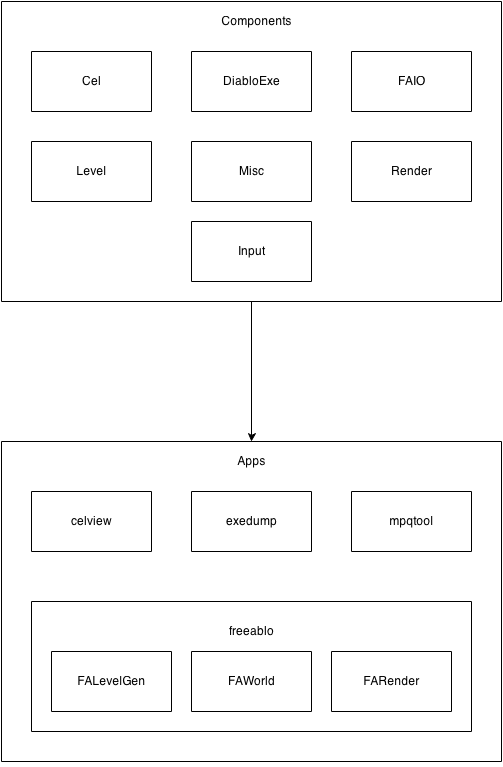
\includegraphics[scale=0.4]{architecture.png}
		\caption{Engine Architecture}
	\end{figure}
	
	\section{Interaction}
	Render and Input are tightly coupled, due to both being supplied by SDL.
	A number of the components use other components (for example, Cel uses FAIO to load the unprocessed image data from the MPQ file).
	Apps are allowed to depend on Components, but not vice-versa.